\begin{enumerate}
\item Find the area of the shaded region in \figref{fig:Fig2}, where arcs drawn with centres $\vec{A,B,C}$ and $\vec{D}$ intersect in pairs at mid-points $\vec{P, Q, R}$ and $\vec{S}$ of the sides AB, BC, CD and DA respectively of a square ABCD of side $12$ cm. ({\textbf{Use}}  $\pi  = 3.14  $)
	\begin{figure}[H]
		\centering
		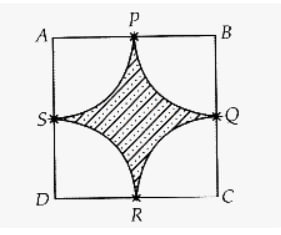
\includegraphics[width=\columnwidth]{figs/squareq20.jpg}
		\caption{square ABCD}
		\label{fig:Fig2}
	\end{figure}
\item A wooden article was made by scooping out a hemisphere from each end of a solid cylinder, as shown in \figref{fig:Fig3}. If the height of the cylinder is $10$ cm and its base is of radius $3.5$ cm. Find the total surface area of the article.
	
	\begin{figure}[H]
		\centering
		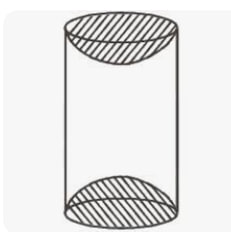
\includegraphics[width=\columnwidth]{figs/cylinderq21.jpg}
		\caption{cylinder}
		\label{fig:Fig3}
	\end{figure} 

	\item A heap of rice is in the form of a cone of base diameter $24$ and height $3.5 m$. Find the volume of the rice. How much canvas cloth is required to just cover the heap?
		\item As observed from the top of a $100 m$ high light house from the sea level, the angles of depression of two ships are $30\degree$ and $45\degree$. If one ship is exactly behind the other on the same side of the light house, find the distance between the two ships. ({\textbf{Use}} $\sqrt3 = 1.732$)
		\item The diameters of the lower and upper ends of a bucket in the form of a frustum of a cone are $10$ cm and $30$ cm respectively. If its height is $24$ cm, find:

			\begin{enumerate}[label=(\roman*)]	
				\item The area of the metal sheet used to make the bucket.
				\item Why we should avoid the bucket made by ordinary plastic? ({\textbf{Use}} $\pi = 3.14 $)
\end{enumerate}
\end{enumerate}
